% ============================================
% CHAPTER 3: PHƯƠNG PHÁP TIẾP CẬN
% ============================================

\chapter{Phương pháp tiếp cận}
\label{chap:methodology}

\section{Tổng quan kiến trúc}
\label{sec:architecture_overview}

% ✅ SƠ ĐỒ KIẾN TRÚC (BẮT BUỘC)

\begin{figure}[H]
\centering
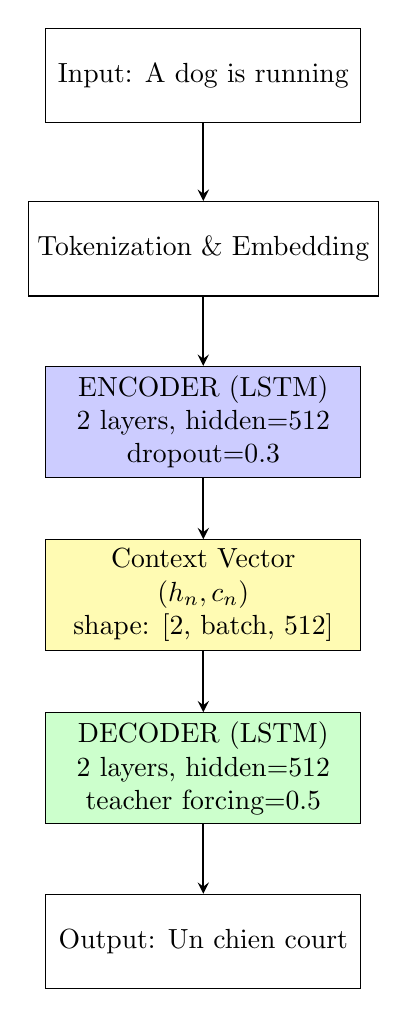
\begin{tikzpicture}[
    node distance=2.2cm,
    box/.style={rectangle, draw, minimum width=4cm, minimum height=1.2cm, align=center},
    arrow/.style={->, >=stealth, thick}
]
    % Input
    \node[box] (input) {Input: A dog is running};
    
    % Tokenization
    \node[box, below of=input] (token) {Tokenization \& Embedding};
    
    % Encoder
    \node[box, below of=token, fill=blue!20] (encoder) {ENCODER (LSTM) \\ 2 layers, hidden=512 \\ dropout=0.3};
    
    % Context vector
    \node[box, below of=encoder, fill=yellow!30] (context) {Context Vector \\ $(h_n, c_n)$ \\ shape: [2, batch, 512]};
    
    % Decoder
    \node[box, below of=context, fill=green!20] (decoder) {DECODER (LSTM) \\ 2 layers, hidden=512 \\ teacher forcing=0.5};
    
    % Output
    \node[box, below of=decoder] (output) {Output: Un chien court};
    
    % Arrows
    \draw[arrow] (input) -- (token);
    \draw[arrow] (token) -- (encoder);
    \draw[arrow] (encoder) -- (context);
    \draw[arrow] (context) -- (decoder);
    \draw[arrow] (decoder) -- (output);
    
\end{tikzpicture}
\caption{Kiến trúc tổng thể LSTM Encoder-Decoder cho dịch máy Anh-Pháp}
\label{fig:architecture}
\end{figure}

Hệ thống dịch máy được xây dựng dựa trên kiến trúc Encoder-Decoder \cite{sutskever2014sequence}, bao gồm 3 thành phần chính:

\begin{enumerate}
    \item \textbf{Encoder}: Mã hóa câu nguồn (tiếng Anh) thành context vector
    \item \textbf{Context Vector}: Vector biểu diễn cố định chứa thông tin của câu nguồn
    \item \textbf{Decoder}: Sinh ra câu đích (tiếng Pháp) từ context vector
\end{enumerate}

\section{Xử lý dữ liệu}
\label{sec:data_processing}

\subsection{Dataset}

Đồ án sử dụng Multi30K dataset \cite{elliott2016multi30k}, corpus song song Anh-Pháp cho domain mô tả hình ảnh.

\begin{table}[H]
\centering
\caption{Thống kê Multi30K dataset}
\label{tab:dataset_stats}
\begin{tabular}{@{}lccc@{}}
\toprule
\textbf{Tập dữ liệu} & \textbf{Số câu} & \textbf{Độ dài TB (EN)} & \textbf{Độ dài TB (FR)} \\ 
\midrule
Training & 29,000 & 13.2 tokens & 14.8 tokens \\
Validation & 1,014 & 13.5 tokens & 15.1 tokens \\
Test & 1,000 & 12.8 tokens & 14.3 tokens \\
\bottomrule
\end{tabular}
\end{table}

\subsection{Tokenization}

Sử dụng tokenization dựa trên regex, bao gồm:
\begin{itemize}
    \item Chuyển về lowercase
    \item Tách punctuation: \texttt{"don't"} $\rightarrow$ \texttt{["do", "n't"]}
    \item Giữ nguyên số và ký tự đặc biệt
\end{itemize}

\textbf{Ví dụ:}
\begin{lstlisting}[language=Python, caption={Tokenization example}]
Input:  "A dog is running!"
Output: ["a", "dog", "is", "running", "!"]
\end{lstlisting}

\subsection{Vocabulary}

Xây dựng vocabulary riêng cho mỗi ngôn ngữ:
\begin{itemize}
    \item \textbf{Max size}: 15,000 từ phổ biến nhất
    \item \textbf{Min frequency}: Giữ tất cả từ (min\_freq=1)
    \item \textbf{Special tokens}:
    \begin{itemize}
        \item \texttt{<pad>} (index=0): Padding token
        \item \texttt{<unk>} (index=1): Unknown token
        \item \texttt{<sos>} (index=2): Start of sequence
        \item \texttt{<eos>} (index=3): End of sequence
    \end{itemize}
\end{itemize}

\subsection{Padding và Packing}

Để xử lý batch có độ dài khác nhau, sử dụng:
\begin{enumerate}
    \item \textbf{Padding}: Thêm \texttt{<pad>} để các câu có cùng độ dài
    \item \textbf{Sorting}: Sắp xếp giảm dần theo độ dài (yêu cầu của \texttt{pack\_padded\_sequence})
    \item \textbf{Packing}: Loại bỏ padding token khỏi computation để tăng tốc
\end{enumerate}

\section{Mô hình Encoder}
\label{sec:encoder_model}

Encoder sử dụng LSTM 3 lớp để mã hóa câu nguồn.

\textbf{Công thức LSTM cell:}
\begin{align}
f_t &= \sigma(W_f [h_{t-1}, x_t] + b_f) \quad \text{(forget gate)} \\
i_t &= \sigma(W_i [h_{t-1}, x_t] + b_i) \quad \text{(input gate)} \\
\tilde{c}_t &= \tanh(W_c [h_{t-1}, x_t] + b_c) \quad \text{(candidate)} \\
c_t &= f_t \odot c_{t-1} + i_t \odot \tilde{c}_t \quad \text{(cell state)} \\
o_t &= \sigma(W_o [h_{t-1}, x_t] + b_o) \quad \text{(output gate)} \\
h_t &= o_t \odot \tanh(c_t) \quad \text{(hidden state)}
\end{align}

\textbf{Kiến trúc Encoder:}
\begin{lstlisting}[language=Python, caption={Encoder implementation}]
class Encoder(nn.Module):
    def __init__(self, vocab_size, emb_dim, hid_dim, 
                 n_layers, dropout):
        super().__init__()
        self.embedding = nn.Embedding(vocab_size, emb_dim, 
                                       padding_idx=0)
        self.lstm = nn.LSTM(emb_dim, hid_dim, n_layers,
                            dropout=dropout if n_layers > 1 else 0)
        self.dropout = nn.Dropout(dropout)
        
    def forward(self, src, src_len):
        # src: [src_len, batch_size]
        embedded = self.dropout(self.embedding(src))
        # embedded: [src_len, batch_size, emb_dim]
        
        packed = pack_padded_sequence(embedded, src_len.cpu())
        outputs, (hidden, cell) = self.lstm(packed)
        # hidden, cell: [n_layers, batch_size, hid_dim]
        
        return hidden, cell  # Context vector
\end{lstlisting}

\section{Mô hình Decoder}
\label{sec:decoder_model}

Decoder nhận context vector từ Encoder và sinh ra câu đích từng token một.

\textbf{Teacher Forcing (Scheduled Sampling):}
\begin{itemize}
    \item Trong training: Bắt đầu với xác suất 70\%, giảm dần xuống 50\% (scheduled sampling)
    \item Giúp model hội tụ nhanh hơn, nhưng có thể gây exposure bias
    \item Scheduled sampling giúp giảm exposure bias trong quá trình training
\end{itemize}

\textbf{Kiến trúc Decoder:}
\begin{lstlisting}[language=Python, caption={Decoder implementation}]
class Decoder(nn.Module):
    def __init__(self, vocab_size, emb_dim, hid_dim, 
                 n_layers, dropout):
        super().__init__()
        self.vocab_size = vocab_size
        self.embedding = nn.Embedding(vocab_size, emb_dim)
        self.lstm = nn.LSTM(emb_dim, hid_dim, n_layers,
                            dropout=dropout if n_layers > 1 else 0)
        self.fc_out = nn.Linear(hid_dim, vocab_size)
        self.dropout = nn.Dropout(dropout)
        
    def forward(self, input, hidden, cell):
        # input: [batch_size]
        input = input.unsqueeze(0)  # [1, batch_size]
        
        embedded = self.dropout(self.embedding(input))
        # embedded: [1, batch_size, emb_dim]
        
        output, (hidden, cell) = self.lstm(embedded, 
                                           (hidden, cell))
        # output: [1, batch_size, hid_dim]
        
        prediction = self.fc_out(output.squeeze(0))
        # prediction: [batch_size, vocab_size]
        
        return prediction, hidden, cell
\end{lstlisting}

\section{Huấn luyện và tối ưu}
\label{sec:training}

\subsection{Hàm mất mát}

Sử dụng Cross-Entropy Loss, bỏ qua padding token:

\begin{equation}
\mathcal{L} = -\sum_{t=1}^{T} \log P(y_t | y_{<t}, x) \cdot \mathbb{1}_{y_t \neq \text{<pad>}}
\end{equation}

\textbf{Trong PyTorch:}
\begin{lstlisting}[language=Python]
criterion = nn.CrossEntropyLoss(ignore_index=PAD_IDX)
\end{lstlisting}

\subsection{Optimizer}

Sử dụng Adam optimizer với learning rate 0.001:

\begin{lstlisting}[language=Python]
optimizer = optim.Adam(model.parameters(), lr=0.001)
\end{lstlisting}

\subsection{Gradient Clipping}

Để tránh exploding gradient, clip gradient norm về max=1:

\begin{lstlisting}[language=Python]
torch.nn.utils.clip_grad_norm_(model.parameters(), 
                               max_norm=1.0)
\end{lstlisting}

\subsection{Early Stopping}

Dừng training nếu validation loss không giảm sau 5 epochs:

\begin{algorithm}[H]
\caption{Early Stopping Algorithm}
\begin{algorithmic}[1]
\STATE best\_val\_loss $\gets \infty$
\STATE patience\_counter $\gets 0$
\FOR{epoch = 1 to max\_epochs}
    \STATE val\_loss $\gets$ evaluate(model, val\_data)
    \IF{val\_loss $<$ best\_val\_loss}
        \STATE best\_val\_loss $\gets$ val\_loss
        \STATE save\_model(model)
        \STATE patience\_counter $\gets 0$
    \ELSE
        \STATE patience\_counter $\gets$ patience\_counter + 1
        \IF{patience\_counter $\geq$ 5}
            \STATE \textbf{break} \COMMENT{Stop training}
        \ENDIF
    \ENDIF
\ENDFOR
\end{algorithmic}
\end{algorithm}

\subsection{Cấu hình huấn luyện}

\begin{table}[H]
\centering
\caption{Siêu tham số huấn luyện}
\label{tab:hyperparameters}
\begin{tabular}{@{}lll@{}}
\toprule
\textbf{Tham số} & \textbf{Giá trị} & \textbf{Lý do chọn} \\ 
\midrule
Embedding dim & 512 & Biểu diễn phong phú hơn \\
Hidden dim & 1024 & Đủ lớn cho phụ thuộc dài và phức tạp \\
Num layers & 3 & Deep LSTM cho biểu diễn tốt hơn \\
Dropout & 0.5 & Regularization mạnh hơn \\
Batch size & 128 & Tối ưu cho GPU T4, tăng throughput \\
Learning rate & 0.001 & Giá trị chuẩn cho Adam \\
Gradient clip & 1.0 & Tránh exploding gradient \\
Teacher forcing & 0.7 $\rightarrow$ 0.5 & Scheduled sampling giảm dần \\
Max epochs & 20 & Với early stopping patience=5 \\
\bottomrule
\end{tabular}
\end{table}
